\chapter{Revisão Bibliográfica}

\begin{justify}

\section{O Complexo Principal de Histocompatibilidade e o Sistema de Antígeno
Leucocitário Humano (HLA)}

O Complexo Maior de Histocompatibilidade (\textit{Major Histocompatibility Complex} - MHC, em inglês) exerce um papel fundamental no sistema imune, responsáveis pela apresentação de peptídeos na superfície celular para reconhecimento das células T \cite{Wieczorek:2017}. A versão humana do MHC , chamado de sistema HLA (\textit{Human Leukocyte Antigen}, em inglês) é codificado a partir do cromossomo 6 e estima-se que apresenta cerca de 40 diferentes genes de HLA, extremamente polimórficos, distribuídos em três classes.  No entanto, apenas duas classes, I e II, estão envolvidas com a resposta imune e possuem diferentes funções e estruturas \cite{Klein:2000}. 

Os genes da Classe I são consideravelmente expressos em células somáticas e dependem do tipo de tecido, já a Classe II está presente nas células do sistema imune incluindo células B, células T ativadas, macrófagos, células dendríticas, etc \cite{Klein:2000, Siegrist:2018}. As Classes I e II também se dividem na localização celular e para entender seu funcionamento é necessário compreender a dinâmica celular no processamento de peptídeos intra- e extracelulares. No citosol, proteínas defeituosas, indesejadas ou desgastadas são processadas pelo proteossoma a partir do reconhecimento da ubiquitina. Esse processamento gera peptídeos que são transportados, com auxílio da classe de Transportadores Associados com o Processamento de Antígenos (TAP, sigla em inglês),  para o retículo endoplasmático e dependendo de sua afinidade de ligação, são reconhecidos pelo MHC Classe I e exportados por meio do Complexo de Golgi até a superfície extracelular (Figura \ref{fig:fig1}A) \cite{Klein:2000}. 

Por outro lado, as proteínas adquiridas do espaçamento extracelular são processadas de maneira diferente. A partir da endocitose (ou fagocitose), as proteínas extracelulares são processadas por meio do mecanismo lisossomal com proteínas proteolíticas para formação de endossomos e reciclagem de aminoácidos. Durante o processamento, o MHC Classe II reconhece os peptídeos pré-processados baseados na afinidade de ligação e são exportados para superfície extracelular (Figura \ref{fig:fig1}B) \cite{Klein:2000}.

Apesar de haver uma diferença funcional e de localização entre as duas classes, seu funcionamento não é restrito às suas atribuições previamente descritas. Em alguns casos, peptídeos extracelulares são processados pela Classe I e peptídeos intracelulares são processados pela Classe II \cite{Klein:2000}.

\begin{wrapfigure}{c}{\textwidth}
    \centering
    \caption{\justifying Processamento dos antígenos para apresentação ao sistema imune. (A) Principal via de geração dos peptídeos para apresentação pelas moléculas HLA Classe I; (B) e Classe II. }
    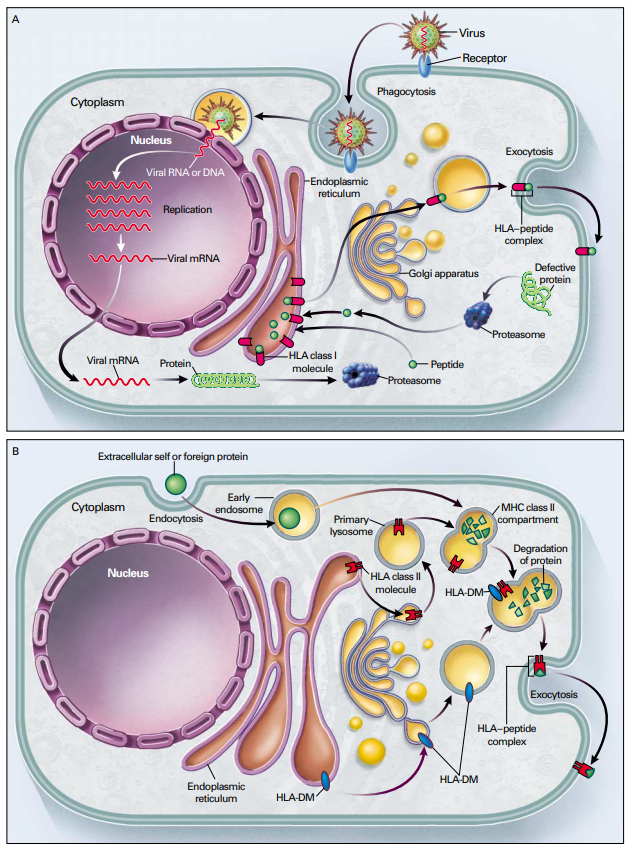
\includegraphics[width=0.7\textwidth]{Figuras/fig1.png}
    \label{fig:fig1}
    \begin{minipage}{0.7\textwidth} % Adjust width as needed
        \centering
        \footnotesize Fonte: \citeonline{Klein:2000}
    \end{minipage}

\end{wrapfigure}

\begin{wrapfigure}{c}{0pt}
\end{wrapfigure}

\section{Estrutura  e Apresentação à Células T}

As estruturas da Classe I e II são compostas por dois domínios, com uma única cadeia-a pesada (Classe I) ou com duas cadeias, cadeia-$\alpha$ e cadeia-$\beta$ (Classe II). Os dois domínios formam uma base folha-$\beta$ e duas $\alpha$-hélices no topo, onde são acomodados os peptídeos. Cada cadeia apresenta um domínio de imunoglobulina, enquanto o MHC Classe I é associado a uma cadeia leve de $\beta$-2 microglobulina ($\beta$2m). Por fim, hélices transmembrana ancoram os complexos na membrana \cite{Wieczorek:2017}.

Os genes que compreendem as Classes I e II apresentam alto grau de polimorfismo (os mais conhecidos são: Classe I: HLA-A, -B, -C; Classe II: HLA-DR, -DP, -DQ), os quais possuem uma variação alélica que afeta a ligação de peptídeos nos sulcos de ligação e modulam a seleção de peptídeos apresentados na superfície celular pelo MHC. No sulco de ligação, a estrutura helicoidal se liga aos peptídeos de acordo com a (i) formação de ligações de hidrogênio entre as estruturas do MHC e o peptídeo e a (ii) ocupação de pequenos espaços que ancoram resíduos da cadeia lateral peptídica \cite{Wieczorek:2017}. Apenas alguns desses pequenos espaços já podem determinar a especificidade de cada peptídeo em se ligar ao complexo e geralmente é definido pela conformação dos diferentes alelos \cite{Klein:2000}.

Essa interação das cadeias laterais de cada peptídeo depende da geometria, distribuição de carga e hidrofobicidade na ligação ao sulco. No entanto, a predição de afinidade nessa interação MHC-antígeno não depende somente das características moleculares, como o tamanho (8-12 resíduos para Classe I e 13-25 resíduos para Classe II) ou composição das cadeias laterais,  se não das conformações transitórias e energéticas das estruturas do MHC durante suas flutuações de equilíbrio da estrutura molecular. Por isso, o carregamento do MHC é influenciado por diferentes fatores, como disponibilidade de antígenos, atividade das proteases, disponibilidade de chaperonas e interação com proteínas auxiliares, como a Tapasina (Classe I) e HLA-DM (Classe II) \cite{Wieczorek:2017}.

A partir da ligação, o MHC é transportado até a superfície celular para apresentação do antígeno para células T. Na região dos linfonodos, as células T CD4+ reconhecem os antígenos apresentados pela Classe II, enquanto as células T CD8+ reconhecem o complexo MHC-peptídeos formados pela Classe I. O reconhecimento dos peptídeos, geralmente, não são o suficiente para ativação das células T, as quais permanecem anérgicas ou se tornam tolerantes na falta de um estímulo secundário \cite{Siegrist:2018}. 

\section{Estrutura e Processo de Infecção de SARS-CoV-2}

O genoma de SARS-COV-2 é composto por 14 ORFs, os quais codificam cerca de 29 proteínas virais. Com aproximadamente 30kb, esse genoma contém inicialmente duas ORFs (ORF1a e ORF1b) responsáveis pela expressão de duas poliproteínas (pp1a e pp1ab) que podem ser processadas em 15-16 proteínas não-estruturais; quatro conjunto de proteínas estruturais (\textit{nucleocapsídeo} (N), \textit{spike} (S), \textit{membrana} (M) e \textit{envelope} (E)); e uma série de proteínas acessórias (\textit{ORF3a, ORF3b, ORF6, ORF7a, ORF7b, ORF8b, ORF9b e ORF14}) \cite{Tay:2020, Vkovski:2021, Yang:2021}.

Na região terminal 5’ estão presentes os genes das poliproteínas, essas proteínas são codificados por duas regiões \textit{ORF1} sobrepostas e são digeridas por duas proteases virais, PL2 e 3CL-pro, resultando em 16 proteínas não-estruturais (NSPs, em inglês), as quais compõe o complexo de  replicação e transcrição viral (RTC).  Enquanto a região terminal 3’ codifica proteínas estruturas e ORFs intercaladas codificam proteínas acessórias com diferentes funções no processo de infecção e montagem do vírion resultante \cite{Vkovski:2021}.

O vírus acessa o espaço intracelular por meio de interações entre a proteína S com receptores celulares e proteínas auxiliares (como a Enzima Conversora da Angiostensina 2 - ACE2 e a proteína transmembrana TMPRSS2, respectivamente) , acarretando na fusão entre a membrana celular do hospedeiro e a viral (Figura \ref{fig:fig2}). A fusão permite a liberação do RNA viral genômico no espaço intracelular que são traduzidas por ribossomos funcionais sequestrados do mecanismo natural da célula hospedeira. Inicialmente, as poliproteínas pp1a e pp1ab são co-expressas e digeridas em NPSs para se agregarem e formarem o RTC \cite{Tay:2020, Yang:2021}.

\begin{wrapfigure}{c}{\textwidth}
    \centering
    \caption{\justifying Etapas do processo de infecção de SARS-CoV-2, incluindo entrada viral, replicação e transcrição, montagem e liberação. }
    \includegraphics[width=0.7\textwidth]{Figuras/fig2.png}
    \label{fig:fig2}
    \begin{minipage}{0.7\textwidth} % Adjust width as needed
        \centering
        \footnotesize Fonte: \citeonline{Yang:2021}
    \end{minipage}

\end{wrapfigure}

\begin{wrapfigure}{c}{0pt}
\end{wrapfigure}

\vspace{10mm}

Durante o ciclo da infecção viral, algumas organelas se auto-replicam a partir do retículo endoplasmático (RE) e propiciam um ambiente favorável para replicação e transcrição de mRNAs subgenômicos (\textit{sg-mRNAs}). Aparentemente, esse mecanismo de replicação é evitado no citosol, provavelmente, para não ser detectado por sensores do sistema imune inato \cite{Vkovski:2021}. As proteínas estruturais que são traduzidas no RE acabam sendo translocadas entre as membranas do RE até o Complexo de Golgi por meio de um compartimento intermediário, onde o vírion resultante é formado.  Por fim, o vírion formado é secretado por exocitose para seguir com o ciclo de infecção nas demais células do hospedeiro \cite{Vkovski:2021, Yang:2021}.



\section{NetMHCpan: Predição de afinidade de ligação entre MHC e antígenos virais}


A identificação de epítopos de células T é um grande desafio devido à significativa variação em seu reconhecimento entre indivíduos. Os genes envolvidos com o sistema HLA são os mais diversos do genoma humano, além dos fatores ambientais que afetam o histórico de interação entre o sistema de apresentação de antígenos. As moléculas de MHC apresentam especificidades de ligação distintas, caracterizando um sistema de apresentação de epítopos robusto e variado. Na Figura \ref{fig:fig3} é possível verificar a quantidade de interações que podem ser geradas a partir da ligação entre o MHC e o peptídeo.

\begin{wrapfigure}{c}{\textwidth}
    \centering
    \caption{\justifying Resíduos âncoras Leucina e Valina de um peptídeo ALGIGILTV na fenda de HLA-A*02:01. }
    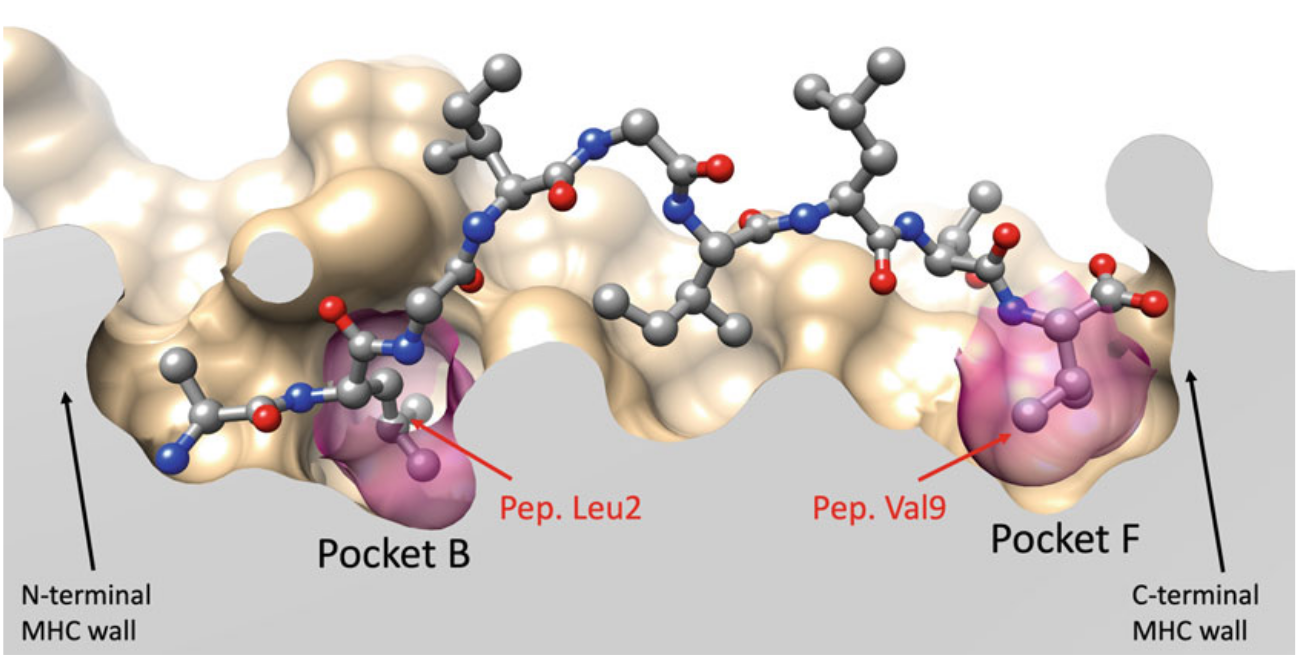
\includegraphics[width=0.7\textwidth]{Figuras/fig3.png}
    \label{fig:fig3}
    \begin{minipage}{0.7\textwidth} % Adjust width as needed
        \centering
        \footnotesize Fonte: \citeonline{Perez:2022}
    \end{minipage}
\end{wrapfigure}

\begin{wrapfigure}{c}{0pt}
\end{wrapfigure}

\vspace{10mm}

A ligação de peptídeos ao MHC é uma etapa necessária para que o sistema imune adaptativo e inato possa ser ativado, esses ligantes são classificados como epítopos de células T. Essa etapa representa o processo mais seletivo da via de reconhecimento de antígenos e compreender os mecanismos que influenciam esse evento contribui para o desenvolvimento de ferramentas, as quais  podem predizer potenciais alvos que ativam ou não uma resposta imune por meio de vias dependentes de MHC \cite{Peters:2020}. 

Essas aplicações corroboram com os avanços no desenvolvimento de vacinas, imunoterapia do câncer e pesquisa de doenças infecciosas. Por isso, múltiplos esforços são aplicados no desenvolvimento de métodos computacionais capazes de acuradamente predizer a ligação de peptídeos e mapear os epítopos ao MHC-I e MHC-II. Entre eles, existem o SYFPEITHI \cite{Rammensee:1999}, netMHCpan \cite{Reynisson:2020}, MHCflurry \cite{Odonnell:2020}, MHCnuggets \cite{Shao:2020} e MixMHCpred \cite{Gfeller:2023}.

De acordo com \citeonline{Peters:2020}, esses métodos computacionais são responsáveis por mapear os epítopos de células T que evoluíram ao longo do tempo, adicionando características a cada versão. Inicialmente, visava-se identificar os \textit{motifs} formados pelos aminoácidos dos peptídeos, os quais correspondiam aos resíduos de ligação ao MHC. Determinadas posições desses peptídeos permitem um limitado número de substituintes e com propriedades de cadeia-laterais semelhantes, os quais mantêm o potencial de ligação MHC-ligante. Esses resíduos foram chamados de resíduos âncoras e outros influentes foram classificados como auxiliares, os quais também possuíam um espaçamento e especificidade determinante para afinidade de ligação que quando somados caracterizavam os motifs dos resíduos ligantes ao MHC (Figura \ref{fig:fig4}A).

Em um segundo momento, esses métodos foram aprimorados para abordagens quantitativas da afinidade de ligação do MHC utilizando abordagens de aprendizado de máquina.  Nesse sentido, uma abordagem inicial foi determinar pontuações, a partir de valores heurísticos, para os vinte aminoácidos em cada posição que quantitativamente representasse o  seu impacto esperado. Esses valores eram estimados a partir de dados experimentais e eram derivados para se obter uma pontuação final de uma sequência peptídica em relação à determinada variante de MHC. A partir da eficiência do método heurístico, abordagens baseadas em aprendizado de máquina supervisionado foram implementadas (Figura \ref{fig:fig4}B).

Em uma terceira abordagem, as atuais ferramentas utilizam arquiteturas de redes neurais artificiais especializadas para integrar informações das interações lineares e não-lineares a partir da sequência do MHC e dados da ligação MHC-ligante. No entanto, dados experimentais são um limitante para o treinamento supervisionado, dado o número de variantes existentes. Essa limitação motivou o desenvolvimento de técnicas que baseiam-se na construção de matrizes virtuais que caracterizam o perfil de ligação de determinada variante de MHC, sem dados experimentais, por meio da comparação  dos resíduos do sulco de ligação do MHC com os resíduos do sulco de ligação de variantes que foram avaliados experimentalmente. Essa última abordagem ficou conhecida como \textit{pan-specific}, exibindo alta confiabilidade na predição de epítopos  para variantes MHC sem dados experimentais (Figura \ref{fig:fig4}C).

\begin{wrapfigure}{c}{\textwidth}
    \centering
    \caption{\justifying Representação das metodologia computacionais desenvolvidas para predição de epítopos de células T baseada em (A) \textit{motifs}, (B) métodos quantitativos heurísticos e (C) redes neurais artificiais.  }
    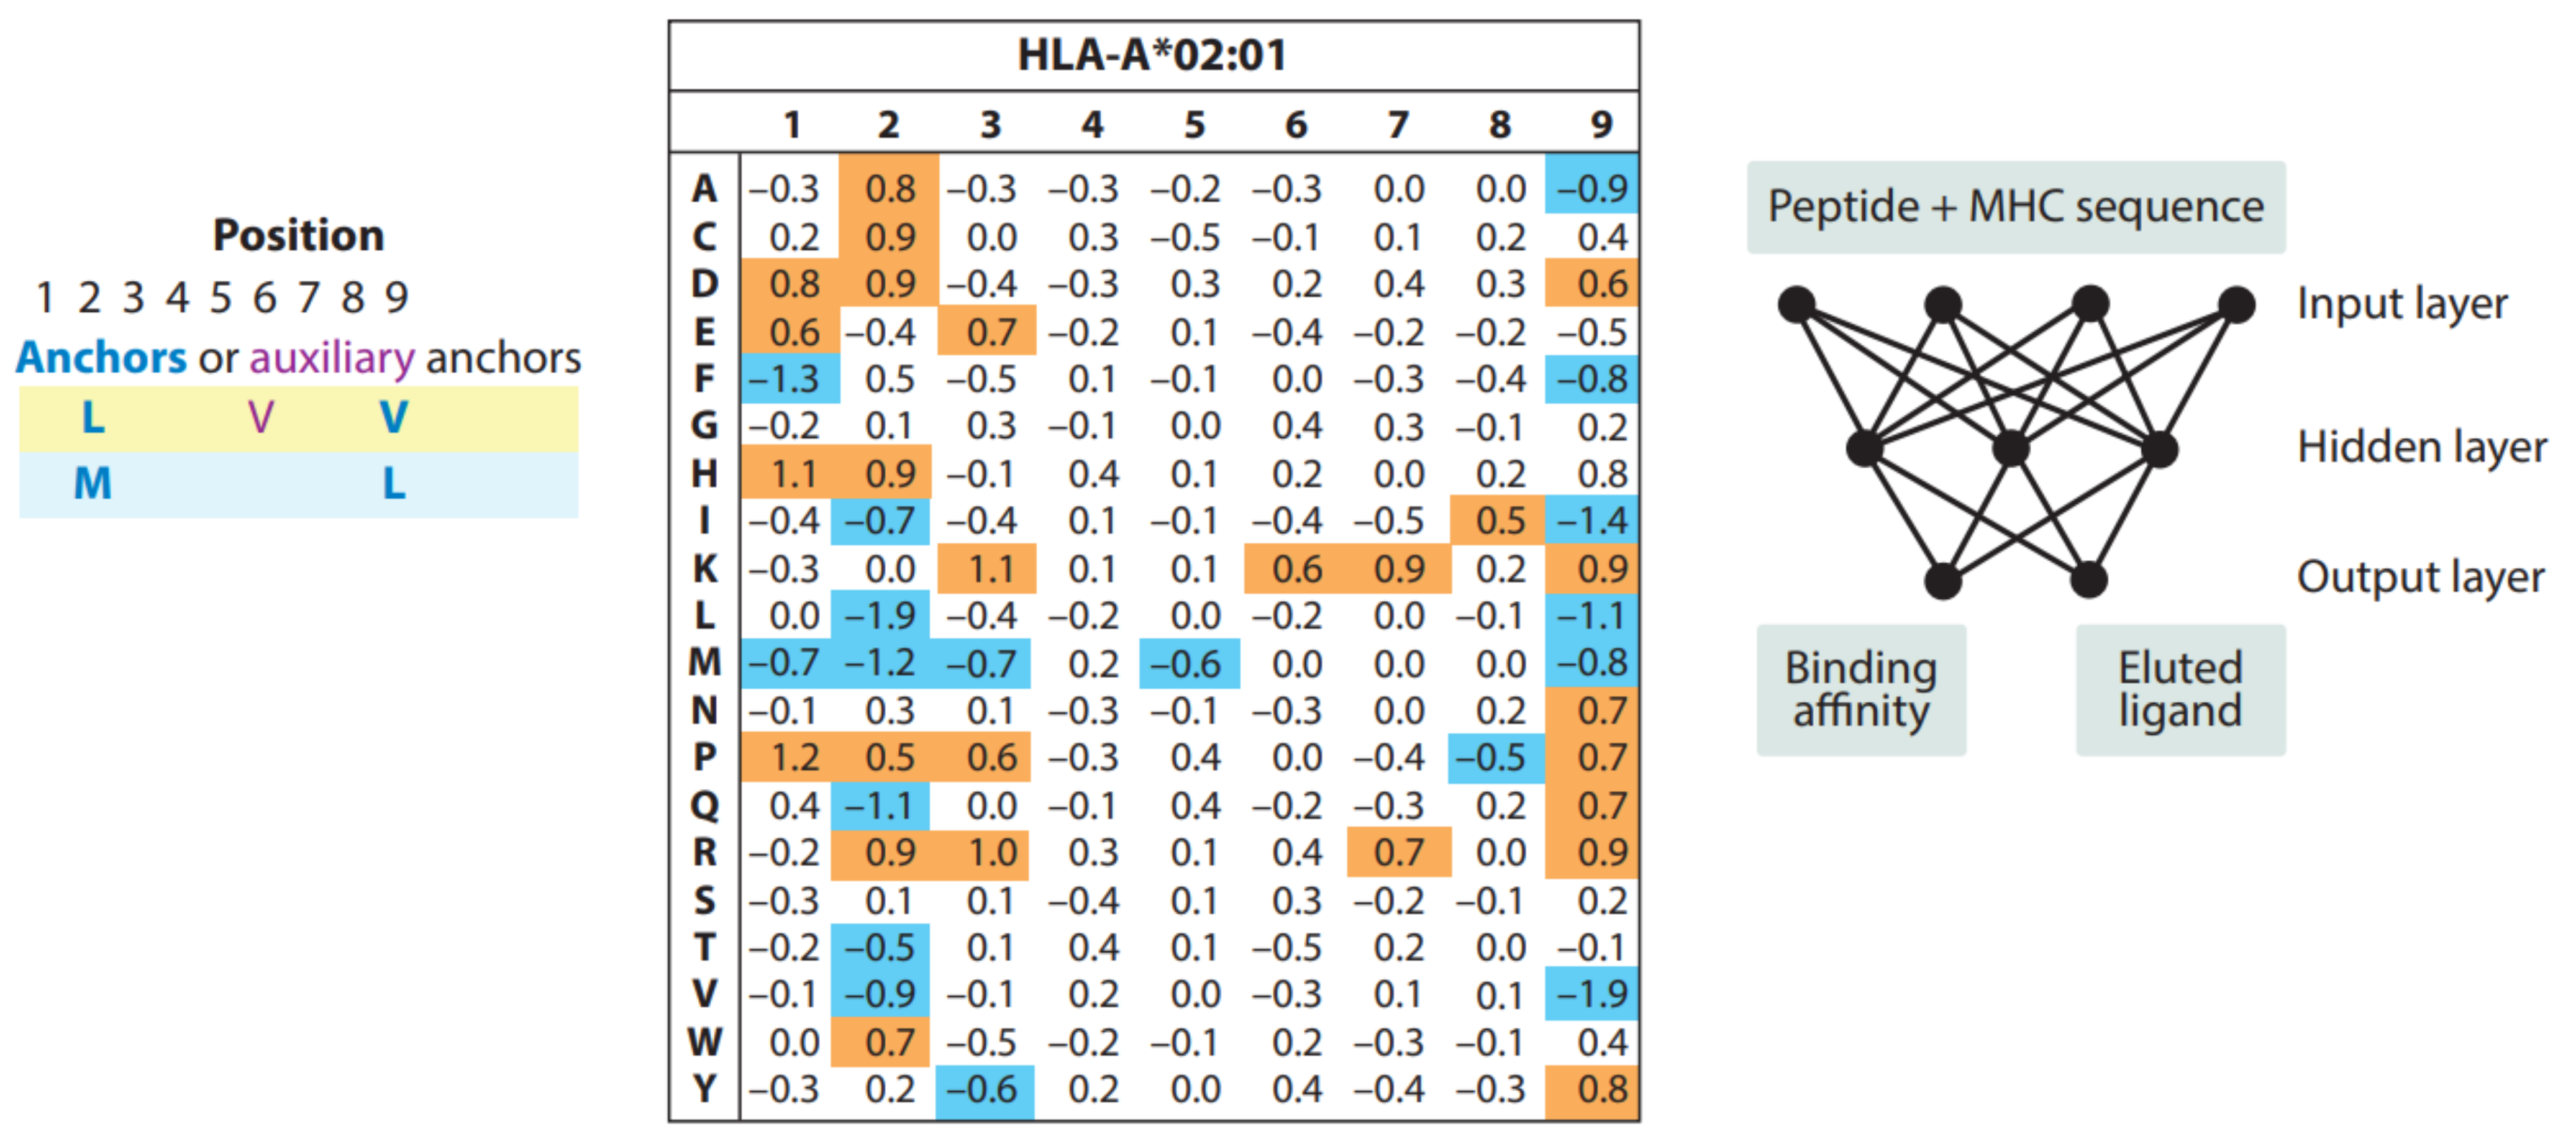
\includegraphics[width=0.7\textwidth]{Figuras/fig4.png}
    \label{fig:fig4}
    \begin{minipage}{0.7\textwidth} % Adjust width as needed
        \centering
        \footnotesize Fonte: \citeonline{Peters:2020}
    \end{minipage}
\end{wrapfigure}

\begin{wrapfigure}{c}{0pt}
\end{wrapfigure}

\vspace{10mm}

O primeiro método computacional a implementar predições \textit{pan-specific}  em redes neurais para moléculas do MHC Classe I foi o NetMHCpan \cite{Hoof:2009}. Esse método complementa a informação sobre a ligação MHC-ligante e ligante eluído no treinamento do modelo preditivo com informações sobre os aminoácidos que definem o sulco de ligação do MHC. Além disso, a partir de aprimoramentos, o NetMHCpan-4.1 permite desambiguar peptídeos que tiveram baixa resolução de anotação para determinados alelos a partir de dados experimentais e aumento a performance de predição em relação à demais ferramentas \cite{Reynisson:2020}.

Portanto, nesse trabalho, busca-se implementar a ferramenta NetMHCpan-4.1 na avaliação dos efeitos na ligação entre peptídeo-MHC a partir dos dados de mutações \textit{missense} de variantes de SARS-CoV-2 identificadas em Foz do Iguaçu/PR. 

\end{justify}


